% flashcards-title: Unlabeled symmetric interval
% flashcards-desc: A high-contrast number-line segment has two bracket endpoints and a distinct gold marker exactly at its center. No numerical endpoint labels are shown.
\documentclass[border=5mm]{standalone}
\def\pgfsysdriver{pgfsys-dvisvgm.def}
\usepackage{tikz}
\usetikzlibrary{arrows.meta,calc,patterns.meta,positioning}
\renewcommand{\familydefault}{\sfdefault}

\definecolor{fcInk}{HTML}{1C1C1E}
\definecolor{fcMuted}{HTML}{68686D}
\definecolor{fcGuide}{HTML}{C9C9CE}
\definecolor{fcGold}{HTML}{D7A313}
\definecolor{fcGoldSoft}{HTML}{F8E8AE}

\tikzset{
  fc canvas/.style={fill=white, rounded corners=2.5mm},
  fc vector/.style={
    draw=fcGold,
    line width=1.35mm,
    line cap=round,
    -{Stealth[length=4.1mm,width=3.25mm]}
  },
  fc vector secondary/.style={
    draw=fcInk,
    line width=1.15mm,
    line cap=round,
    dash pattern=on 4.1mm off 2.6mm,
    -{Stealth[length=3.9mm,width=3.1mm]}
  },
  fc resultant/.style={
    draw=fcMuted,
    line width=1.55mm,
    line cap=round,
    -{Stealth[length=4.6mm,width=3.6mm]}
  },
  fc axis/.style={
    draw=fcInk,
    line width=.72mm,
    -{Stealth[length=3.1mm,width=2.5mm]}
  },
  fc guide/.style={
    draw=fcMuted,
    line width=.55mm,
    dash pattern=on 2.3mm off 1.8mm
  },
  fc construction/.style={draw=fcGuide, line width=.32mm},
  fc endpoint/.style={circle, fill=fcInk, inner sep=1.45mm},
  fc label/.style={font=\bfseries\large, text=fcInk},
  fc small label/.style={font=\small, text=fcMuted},
  fc caption/.style={font=\bfseries\small, text=fcMuted}
}

\begin{document}
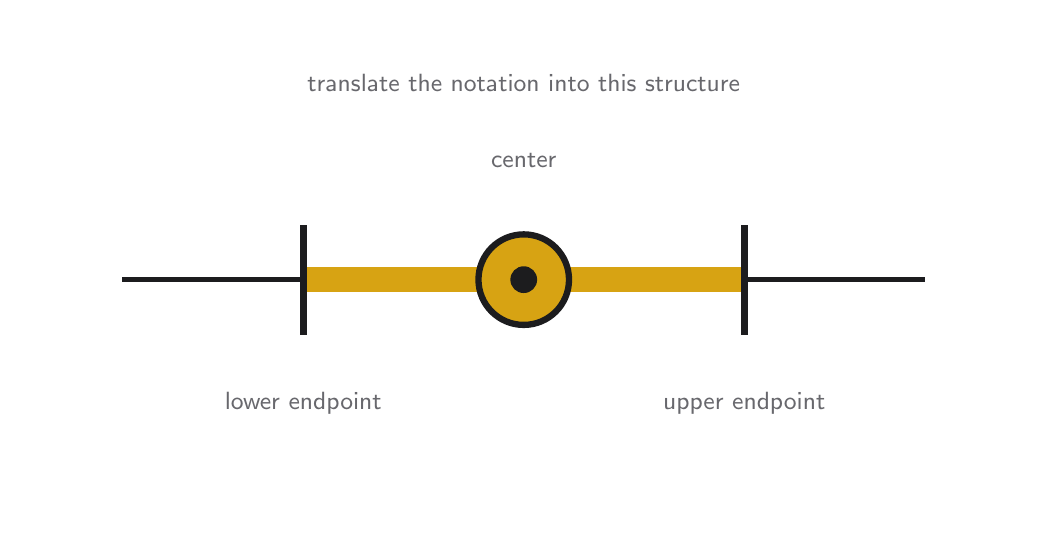
\begin{tikzpicture}[x=1cm,y=1cm]
  \path[fc canvas] (-.45,-.45) rectangle (12.15,5.95);
  \node[fc small label] at (5.85,5.25) {translate the notation into this structure};

  \draw[draw=fcInk, line width=.72mm] (.75,2.75) -- (10.95,2.75);
  \draw[draw=fcGold, line width=3.2mm] (3.05,2.75) -- (8.65,2.75);
  \draw[draw=fcInk, line width=.92mm] (3.05,2.05) -- (3.05,3.45)
    (8.65,2.05) -- (8.65,3.45);
  \node[circle, draw=fcInk, fill=fcGold, line width=.8mm,
    minimum size=11.5mm] (estimate) at (5.85,2.75) {};
  \node[circle, fill=fcInk, minimum size=3.4mm, inner sep=0] at (estimate) {};

  \node[fc small label, below=6mm] at (3.05,2.05) {lower endpoint};
  \node[fc small label, above=6mm] at (5.85,3.45) {center};
  \node[fc small label, below=6mm] at (8.65,2.05) {upper endpoint};
\end{tikzpicture}
\end{document}
